In order to study the effect of the variations of the frequency $f_c$ and the amplitude $A_u$ of the input $u_e$ on the second and third order harmonic distortion, we have computed $d_2$ and $d_3$ for a range of $A_u$ and $f_c$. The results can be seen on the figure \ref{fig:d2d3}. According to the graphic, the variations of the amplitude of the input do not affect the distortion levels. On the opposite, when the fundamental frequency increases, the distortion level 

\begin{figure}[H]
 \centering 
 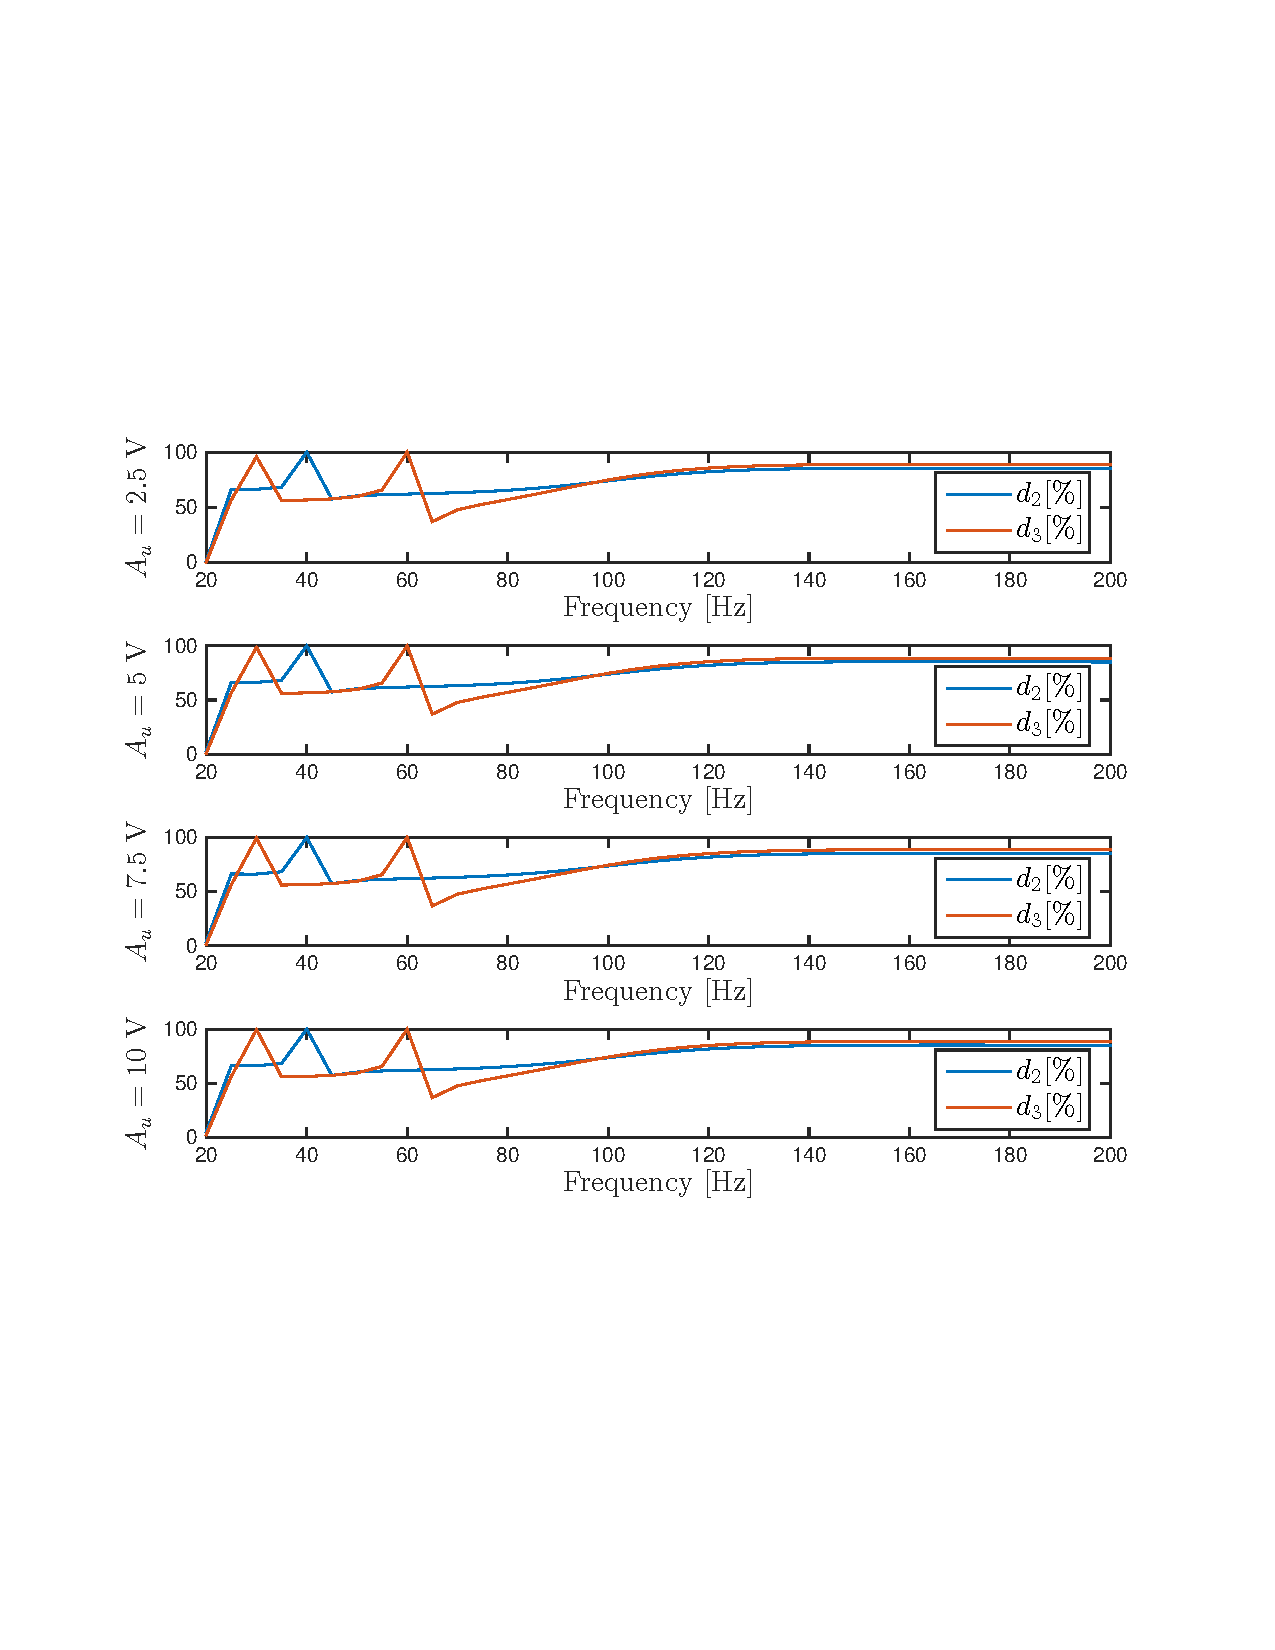
\includegraphics[trim=2cm 7cm 2cm 7cm, clip=true, totalheight=0.35\textheight, angle=0]{figures/d2d3.pdf}
 \caption{Effect of the variations of the frequency $f_c$ and the amplitude $A_u$ of the input $u_e$ on the second and third order harmonic distortion}
 \label{fig:d2d3}
\end{figure}